181. \begin{figure}[ht!]
\center{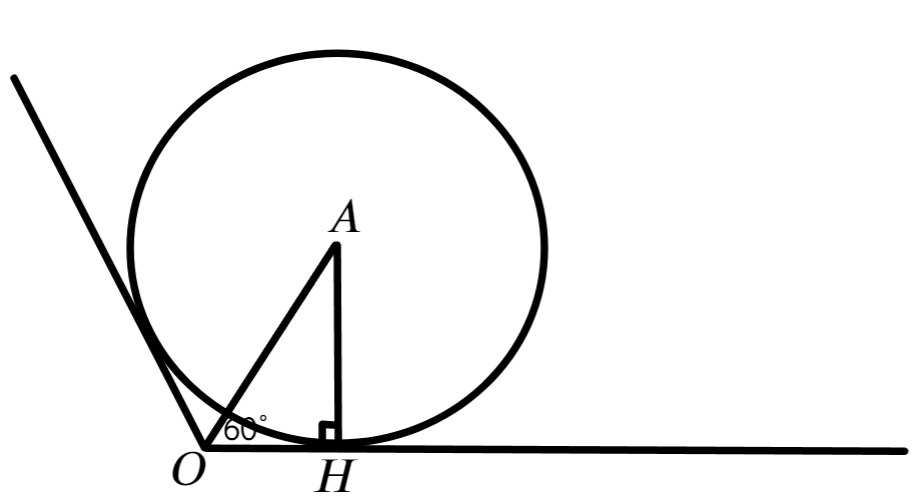
\includegraphics[scale=0.35]{g9-181.png}}
\end{figure}\\
Опустим из центра круга $A$ перпендикуляр $AH.$ Так как центр круга равноудалён от сторон угла, он лежит на его биссектрисе, поэтому $\angle AOH=120^\circ:2=60^\circ.$ Если площадь круга равна $81\pi,$ то $\pi r^2=81\pi,\ r=9.$ Значит, $AH=9$ и $OA=\cfrac{9}{\sin(60^\circ)}=\cfrac{9}{\cfrac{\sqrt{3}}{2}}=6\sqrt{3}.$\\
